
\subsection{Graphs Encoding Algebraic Expressions}\label{subsec:alg_graph_exp}

We will now describe a method of encoding expressions involving tensor products,
point-wise algebra products and composition of linear maps $A \to A$ for some
algebra $A$, using directed graphs. As a matter of convention, we will take all
graphs to mean directed acyclic graphs where we do not allow parallel edges or
self-loops, unless stated otherwise. However, we do allow the underlying
undirected graph of any directed graph to be a forest. Given a graph
$G = (V, E)$, we will write $V = V(G)$ and $E = E(G)$. We now see a motivating
example.

\begin{exm}\label{exm:egraph1}
Consider a graph consisting of nine vertices $1, \dots, 9$ with edges:
\[\begin{array}{ccccc}
  (1, 3) &,& (1, 4) &,& (2, 3),\\
  (3, 5) &,& (3, 6) &,& (4, 7),\\
  (5, 8) &,& (6, 9) &,& (7, 9)
\end{array}\]
We visualize this graph as follows:
\[\begin{tikzpicture}[xscale=2,yscale=0.5]
\node at (0, 3) (v1) {1};
\node at (0, 1) (v2) {2};
\node at (1, 3) (v3) {3};
\node at (1, 1) (v4) {4};
\node at (2, 4) (v5) {5};
\node at (2, 2) (v6) {6};
\node at (2, 0) (v7) {7};
\node at (3, 3) (v8) {8};
\node at (3, 1) (v9) {9};
\midarrow{v1}{v3}
\midarrow[0.33]{v1}{v4}
\midarrow[0.33]{v2}{v3}
\midarrow{v3}{v5}
\midarrow{v3}{v6}
\midarrow{v4}{v7}
\midarrow{v5}{v8}
\midarrow{v6}{v9}
\midarrow{v7}{v9}
\end{tikzpicture}\]
Thinking of individual edges in the above graph as mappings $A \to A$ of some
monoid and comonoid $A$ in some monoidal category, we can think of multiple
incoming edges on a vertex -- for example, the incoming edges on $3$ -- as a
multiplication $\cwedge$ of maps and multiple outgoing edges -- for example, the
outgoing edges of $1$ -- as a comultiplication $\cvee$ of maps. Parallel edges,
multiplications or comultiplications with disjoint sources and targets can be
thought of as a tensor product of maps. We can treat a single vertex as an
identity mapping.

We can then modify the graph as follows:
\[\begin{tikzpicture}[xscale=2,yscale=0.75]
\node at (-2, 3) (v1) {1};
\node at (-2, 1) (v2) {2};
\node at (-1, 4) (v33) {3};
\node at (-1, 2) (v44) {4};
\node at (-1, 1) (v22) {2};
\node at (0, 4) (v333) {3};
\node at (0, 2) (v3333) {3};
\node at (0, 1) (v444) {4};
\node at (1, 3) (v3) {3};
\node at (1, 1) (v4) {4};
\node at (2, 4) (v5) {5};
\node at (2, 2) (v6) {6};
\node at (2, 0) (v7) {7};
\node at (3, 3) (v8) {8};
\node at (3, 1) (v9) {9};
\midarrow{v1}{v33}
\midarrow{v1}{v44}
\midarrow{v2}{v22}
\midarrow{v33}{v333}
\midarrow[0.33]{v22}{v3333}
\midarrow[0.33]{v44}{v444}
\midarrow{v333}{v3}
\midarrow{v3333}{v3}
\midarrow{v444}{v4}
\midarrow{v3}{v5}
\midarrow{v3}{v6}
\midarrow{v4}{v7}
\midarrow{v5}{v8}
\midarrow{v6}{v9}
\midarrow{v7}{v9}
\end{tikzpicture}\]
Thinking of edges between copies of the same vertex, which did not originally
exist, as the identity map and crossing edges as a twist operation -- denoted
$\boxtimes$ -- of maps, we can capture the graph into an algebraic expression of
the following form:
\begin{align*}
        & ((5, 8) \tensor ((6, 9) \cwedge (7, 9))) \\
  \circ & (((3, 5) \cvee (3, 6)) \tensor (4, 7)) \\
  \circ & (((3, 3) \cwedge (3, 3)) \tensor (4, 4)) \\
  \circ & ((3, 3) \tensor ((4, 4) \boxtimes (2, 3))) \\
  \circ & (((1, 3) \cvee (1, 4)) \tensor (2, 2))
\end{align*}

Observe that we have taken a directed acyclic graph and converted it to a
diagram in $\Cob_{2}$ -- the symmetric monoidal category of cobordisms of
dimension $2$. This, in turn, yields an expression involving operations on
endomorphisms of a monoid in some monoidal category. However, we should note
that this is just one possible interpretation of the graph above.
\end{exm}

This motivates us to define an algorithm for extracting expressions from a
directed acyclic graph such as the one above.
\begin{alg}[Expression Construction]
Let $G = (V, E)$ be any graph. We make the following modifications to $G$:
\begin{enumerate}
\setlength{\itemsep}{0pt}

\item For each vertex $v$, choose an ordering of the incoming edges of $v$, say
$(u_1, v), \dots, (u_k, v)$ and an ordering of its outgoing edges, say
$(v, w_1), \dots, (v, w_n)$.

\item Let $S(G)$ be the set consisting of vertices with no incoming
edges -- called the source vertices of $G$ -- and $T(G)$, the set consisting of
vertices with no outgoing edges -- called the target vertices of $G$. We then
choose an ordering of $S(G)$. Note that $S(G) \cap T(G)$ might be non-empty
because of vertices with no edges, incoming or outgoing -- these will be called
the edgeless vertices.

\item Copy vertices and add edges to make the following modification, where the
incoming edges are in order from the lowest at the top to the highest at the
bottom:
\[\begin{tikzpicture}
\node at (2, 0)     (v) {$v$};
\node at (0, 1)     (u1) {$u_1$};
\node at (0, 0.5)   (u2) {$u_2$};
\node at (0, 0)     (u3) {$u_3$};
\node at (0, -1)    (uk) {$u_k$};
\midarrow{u1}{v}
\midarrow{u2}{v}
\midarrow{u3}{v}
\midarrow{uk}{v}
\draw[thick, loosely dotted] (u3) -- (uk);
\end{tikzpicture}
\qquad
\begin{tikzpicture}
\node at (0, 1)   (TOP)     {};
\node at (0, 0)   (TO)      {$\Longrightarrow$};
\node at (0, -1)  (BOTTOM)  {};
\end{tikzpicture}
\qquad
\begin{tikzpicture}
\node at (4, -1)     (v) {$v$};
\node at (0, 1)     (u1) {$u_1$};
\node at (0, 0.5)   (u2) {$u_2$};
\node at (0, 0)     (u3) {$u_3$};
\node at (0, -1)    (uk) {$u_k$};
\node at (1, 0.5) (a)  {$v$};
\node at (2, 0)   (b)  {$v$};
\midarrow{u1}{a}
\midarrow{u2}{a}
\midarrow{a}{b}
\midarrow{u3}{b}
\draw[thick, loosely dotted] (b) -- (v);
\draw[thick, loosely dotted] (u3)   -- (uk);
\midarrow{uk}{v};
\end{tikzpicture}
\]

\item Copy vertices and edges to make the following modification similar to the
previous step:
\[
\begin{tikzpicture}
\node at (-2, 0)     (v) {$v$};
\node at (0, 1)     (w1) {$w_1$};
\node at (0, 0.5)   (w2) {$w_2$};
\node at (0, 0)     (w3) {$w_3$};
\node at (0, -1)    (wk) {$w_k$};
\midarrow{v}{w1}
\midarrow{v}{w2}
\midarrow{v}{w3}
\midarrow{v}{wk}
\draw[thick, loosely dotted] (u3) -- (uk);
\end{tikzpicture}
\qquad
\begin{tikzpicture}
\node at (0, 1)   (TOP)     {};
\node at (0, 0)   (TO)      {$\Longrightarrow$};
\node at (0, -1)  (BOTTOM)  {};
\end{tikzpicture}
\qquad
\begin{tikzpicture}
\node at (-4, -1)   (v)  {$v$};
\node at (0, 1)     (w1) {$w_1$};
\node at (0, 0.5)   (w2) {$w_2$};
\node at (0, 0)     (w3) {$w_3$};
\node at (0, -1)    (wk) {$w_k$};
\node at (-1, 0.5) (a)  {$v$};
\node at (-2, 0)   (b)  {$v$};
\midarrow{a}{w1}
\midarrow{a}{w2}
\midarrow{b}{a}
\midarrow{b}{w3}
\draw[thick, loosely dotted] (b) -- (v);
\draw[thick, loosely dotted] (w3)   -- (wk);
\midarrow{v}{wk};
\end{tikzpicture}
\]

\item At this point, every vertex has both indegree and outdegree at most $2$.
The chosen edge orderings induces a local geometric orientation -- in an
informal sense -- on the graph. By this we mean, that this allows us to
distinguish the following diagrams in a precise sense:
\[
\begin{tikzpicture}
\node at (0, 0) (u) {$u$};
\node at (2, 0.5) (v) {$v$};
\node at (2, -0.5) (w) {$w$};
\midarrow{u}{v}
\midarrow{u}{w}
\end{tikzpicture}
\qquad
\qquad
\begin{tikzpicture}
\node at (0, 0) (u) {$u$};
\node at (2, -0.5) (v) {$v$};
\node at (2, 0.5) (w) {$w$};
\midarrow{u}{v}
\midarrow{u}{w}
\end{tikzpicture}
\]

The distinction is that if we take $(u, v) < (u, w)$ in the left picture, say,
then we can take $(u, v) > (u, w)$ in the right picture.
Then, for every edge that is shared between a ``multiplication'' and a
``comultiplication'', considering the edge orderings chosen before, we have the
following possibilities for common edges and we make the modifications shown:
\[
\begin{tikzpicture}
\node at (0, 2) (u) {$u$};
\node at (2, 2) (v) {$v$};
\node at (0, 0) (w) {$w$};
\node at (2, 0) (x) {$x$};
\midarrow{u}{v}
\midarrow{u}{x}
\midarrow{w}{x}
\end{tikzpicture}
\qquad
\begin{tikzpicture}
\node at (0, 1)   (TOP)     {};
\node at (0, 0)   (TO)      {$\Longrightarrow$};
\node at (0, -1)  (BOTTOM)  {};
\end{tikzpicture}
\qquad
\begin{tikzpicture}
\node at (0, 2) (u) {$u$};
\node at (2, 2) (a) {$v$};
\node at (4, 2) (v) {$v$};
\node at (2, 1) (b) {$x$};
\node at (0, 0) (w) {$w$};
\node at (2, 0) (c) {$w$};
\node at (4, 0) (x) {$x$};
\midarrow{u}{a}
\midarrow{a}{v}
\midarrow{u}{b}
\midarrow{b}{x}
\midarrow{w}{c}
\midarrow{c}{x}
\end{tikzpicture}
\]
\[
\begin{tikzpicture}
\node at (0, 0) (u) {$u$};
\node at (1, 2) (v) {$v$};
\node at (2, 0) (w) {$w$};
\midarrow{u}{v}
\midarrow{v}{w}
\midarrow{u}{w}
\end{tikzpicture}
\qquad
\begin{tikzpicture}
\node at (0, 1)   (TOP)     {};
\node at (0, 0)   (TO)      {$\Longrightarrow$};
\node at (0, -1)  (BOTTOM)  {};
\end{tikzpicture}
\qquad
\begin{tikzpicture}
\node at (0, 1) (u) {$u$};
\node at (2, 2) (v) {$v$};
\node at (2, 0) (a) {$w$};
\node at (4, 1) (w) {$w$};
\midarrow{u}{v}
\midarrow{u}{a}
\midarrow{v}{w}
\midarrow{a}{w}
\end{tikzpicture}
\]

\[
\begin{tikzpicture}
\node at (0, 2) (u) {$u$};
\node at (2, 2) (v) {$v$};
\node at (0, 0) (w) {$w$};
\node at (2, 0) (x) {$x$};
\midarrow{u}{v}
\midarrow[0.33]{w}{v}
\midarrow[0.33]{u}{x}
\end{tikzpicture}
\qquad
\begin{tikzpicture}
\node at (0, 1)   (TOP)     {};
\node at (0, 0)   (TO)      {$\Longrightarrow$};
\node at (0, -1)  (BOTTOM)  {};
\end{tikzpicture}
\qquad
\begin{tikzpicture}
\node at (0, 2) (u) {$u$};
\node at (2, 2) (a) {$v$};
\node at (4, 2) (aa) {$v$};
\node at (6, 2) (v) {$v$};
\node at (2, 1) (b) {$x$};
\node at (4, 1) (bb) {$w$};
\node at (0, 0) (w) {$w$};
\node at (2, 0) (c) {$w$};
\node at (4, 0) (cc) {$x$};
\node at (6, 0) (x) {$x$};
\midarrow{u}{a}
\midarrow{u}{b}
\midarrow{w}{c}
\midarrow{a}{aa}
\midarrow[0.33]{b}{cc}
\midarrow[0.33]{c}{bb}
\midarrow{aa}{v}
\midarrow{bb}{v}
\midarrow{cc}{x}
\end{tikzpicture}
\]

We also make the modifications obtained from the rotations of the above diagrams
about a horizontal edge. After these modifications have been applied, there are
no edges shared between ``multiplications'' and ``comultiplications''.

\item Noting that $G$ is acyclic even after the modifications, we construct a
level ordering of $G$ inductively as follows:
\begin{enmrt}
\li Let $V_1$ be the set of vertices with no incoming edges -- i.e.,
$V_1 := S(G)$
\li Let $V_{k + 1}$ be the set of vertices in
$G \setminus (V_1 \cup \cdots \cup V_k)$ with incoming edges only from
$V_1, \dots, V_k$.
\end{enmrt}
We note that the ordering on $S(G) = V_1$ induces an ordering of $V_2$ as
follows. Let $S(G)$ be ordered as $u_1, \dots, u_n$. Let the ordering of the
outgoing edges of $u_i$ be $(u_i, v_{i, 1}), \dots, (u_i, v_{i, k_i})$. We let
$v_i := v_{1, i}$ for $1 \leq i \leq k_1$. For $1 \leq j < n$,
$k_j < i \leq k_{j + 1}$, we let $v_i := v_{j + 1, i}$. Then, the $v_i$ are an
ordering of $V_2$. We can repeat this process with $V_2$ in place of $S(G)$ and
so on to obtain an ordering for each level. By construction, we have the
following corollary:

\begin{cor}\label{cor:lvltolvl}
Let $G$ be an expression graph with induced level ordering
$V_1, V_2, \dots, V_k$. Then for each $i \in \set{2, \dots, k}$ and each
$v \in V_i$ that is not edgeless, there is an edge $(u, v)$ with
$u \in V_{i - 1}$.
\end{cor}

\begin{rmk}
This level ordering algorithm works on any graph -- in particular, on $G$
before the modifications. We will need this construction on arbitrary graphs
later on.
\end{rmk}

\begin{rmk}
The vertices with no edges, incoming or outgoing, are always in the first level.
However, vertices with no outgoing edges need not always be in the last level.
\end{rmk}

\item\label{alg:edgeless}
Consider the vertices with no outgoing edges but not at the last level. For each
such vertex $u$ in $V_i$, we add a copy $u'$, to $V_{i + 1}$. Its insertion
order needs to be made precise. Call the vertices in $V_{i + 1}$ with an
incoming edge from some vertex above $u \in V_{i}$, the vertices above $u$ in
$V_{i + 1}$. Similarly, call the vertices in $V_{i + 1}$ with no incoming edges
from $u$ or a vertex above $u \in V_i$, the vertices below $u$ in $V_{i + 1}$.
A copy of $u$, say $u'$, is inserted
in the position right after the vertices above $u$ and before the vertices below
$u$ in $V_{i + 1}$. We then add in the edge $(u, u')$. We continue this process
with $V_{i + 1}$ in place of $V_i$ and so on, until there is a copy
of $u$ in each level after $V_i$ with a path connecting them.

\begin{rmk}
Each vertex without any edges, incoming or outgoing, are also copied in this
way, noting that these vertices are placed in the first level during the level
ordering.
\end{rmk}

\item For each level skipping edge $(u, v)$ -- that is, with $u \in V_k$ and
$v \in V_{k'}$ for some $k' > k + 1$ -- we insert a copy of $u$ in $V_{i}$ for
each $k < i < k'$ in positions similar to the insertions in the last step. We
call this copy $u'$. We then add an edge $(u, u')$. We repeat this with
$V_{i + 1}$ in place of $V_{i}$ and $u'$ in place of $u$. After this process
completes, we delete the edge $(u, v)$ and add an edge from the copy of $u$
in $V_{k' - 1}$ to $v$. After we complete this process for every
level-skipping edge, level skipping edges are replaced by paths connecting the
source vertex to the target vertex of these edges.

\item Observe that we can now identify the graph $G$ with a cobordism in
$\Cob_2$ from $|S(G)|$ copies of $S^1$ to $|T(G)|$ copies of $S^1$! The
identifications of the generating structures are the obvious ones:
\[
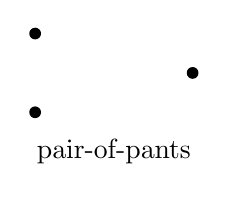
\begin{tikzpicture}
\node[circle, fill, inner sep=1.5pt] at (0, 0) (u) {};
\node[circle, fill, inner sep=1.5pt] at (-2, 0.5) (v) {};
\node[circle, fill, inner sep=1.5pt] at (-2, -0.5) (w) {};
\midarrow{v}{u}
\midarrow{w}{u}
\node at (-1, -1) (lbl) {pair-of-pants};
\end{tikzpicture}
\qquad
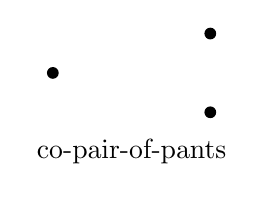
\begin{tikzpicture}
\node[circle, fill, inner sep=1.5pt] at (0, 0) (u) {};
\node[circle, fill, inner sep=1.5pt] at (2, -0.5) (v) {};
\node[circle, fill, inner sep=1.5pt] at (2, 0.5) (w) {};
\midarrow{u}{v}
\midarrow{u}{w}
\node at (1, -1) (lbl) {co-pair-of-pants};
\end{tikzpicture}
\qquad
\begin{tikzpicture}
\node[circle, fill, inner sep=1.5pt] at (0, 0) (u) {};
\node at (2, -0.5) (v) {};
\node at (2, 0.5) (w) {};
\node[circle, fill, inner sep=1.5pt] at (2, 0) (x) {};
\midarrow{u}{x}
\node at (1, -1) (lbl) {cylinder};
\end{tikzpicture}
\]
Note that the cap or cup were not used. This, then, directly yields an
expression of the original graph $G$ similar to the example.

\end{enumerate}
\end{alg}

\begin{defn}[Expression of a Graph]
Given a graph $G$, the expression resulting from the algorithm above is called
an expression of $G$ and denoted $\Exp{G}$.
\end{defn}

\begin{rmk}
Note that an expression of a graph is by no means unique -- we made a large
number of arbitrary choices in our process.
\end{rmk}

\begin{rmk} We also note that we did not specify how to handle ``crossings'' of
edges but it is not difficult to see that ``crossing'' makes precise sense when
we specify the edge orderings and the ordering of the source of a graph. Once we
execute the algorithm above, we can handle crossings in the same way we handle
them when drawing cobordisms in $\Cob_2$.
\end{rmk}

Even though we made many choices in the above algorithm, the only
choices that cannot be thought of as canonical in any way are the chosen edge
orderings and the ordering of the source vertices. We are thus motivated to make
the following definition.

\begin{defn}[Expression Graph]
A graph with a chosen edge ordering and a chosen ordering of its source vertices
is called an expression graph.
\end{defn}

Thus, given an expression graph, we have an algorithm to extract its expression
consistently as long as we keep the other choices in the above algorithm fixed.
We will later see that $\Exp{G}$ is functorial in a suitable sense.

